\section{Implementation}
\label{section:implementation}

The work presented in this paper is part of an effort in applying
recent theorem proving technologies for the design, implementation and
verification of query compilers. In this section, we review the state
of our implementation and go over practical aspects that were omitted
from the main part of the paper. We also report on our experience in
using theorem proving technology for query compiler implementation.

\paragraph*{The Q*cert Compiler}

Figure~\ref{fig:architecture} gives an overview of the full compiler
architecture. Each square box corresponds to an intermediate
representation specified using Coq.
% the Coq proof assistant~\cite{coq}.
The red coloring identifies the
subset of the compiler that is accompanied by mechanically checked
correctness proofs. Those cover all parts described in this paper,
except for the SQL to \NRAEnv translation. The compiler
implementation is automatically generated from the mechanized
specification using Coq's extraction mechanism~\cite{coq:extraction},
ensuring that the compiler matches the specification.

As of this writing, the implementation supports compilation from
JRules (our initial target and the most complete), a fragment of SQL
and OQL, and \NRALambda. It can emit code for execution in JavaScript
or Java, for Spark, and for the Cloudant NoSQL database. In each case,
the emitted code has to be linked with a small runtime library which
implements core operations over the data model (e.g., record
construction/access, collection operations such as flatten, distinct,
etc). The Java and JavaScript backends are useful for testing and also
serve as building blocks for the Spark and Cloudant backends. For
Cloudant, the compiler produces map/reduce views containing JavaScript
code.

% \paragraph*{Architecture}

\begin{figure}
  \centerline{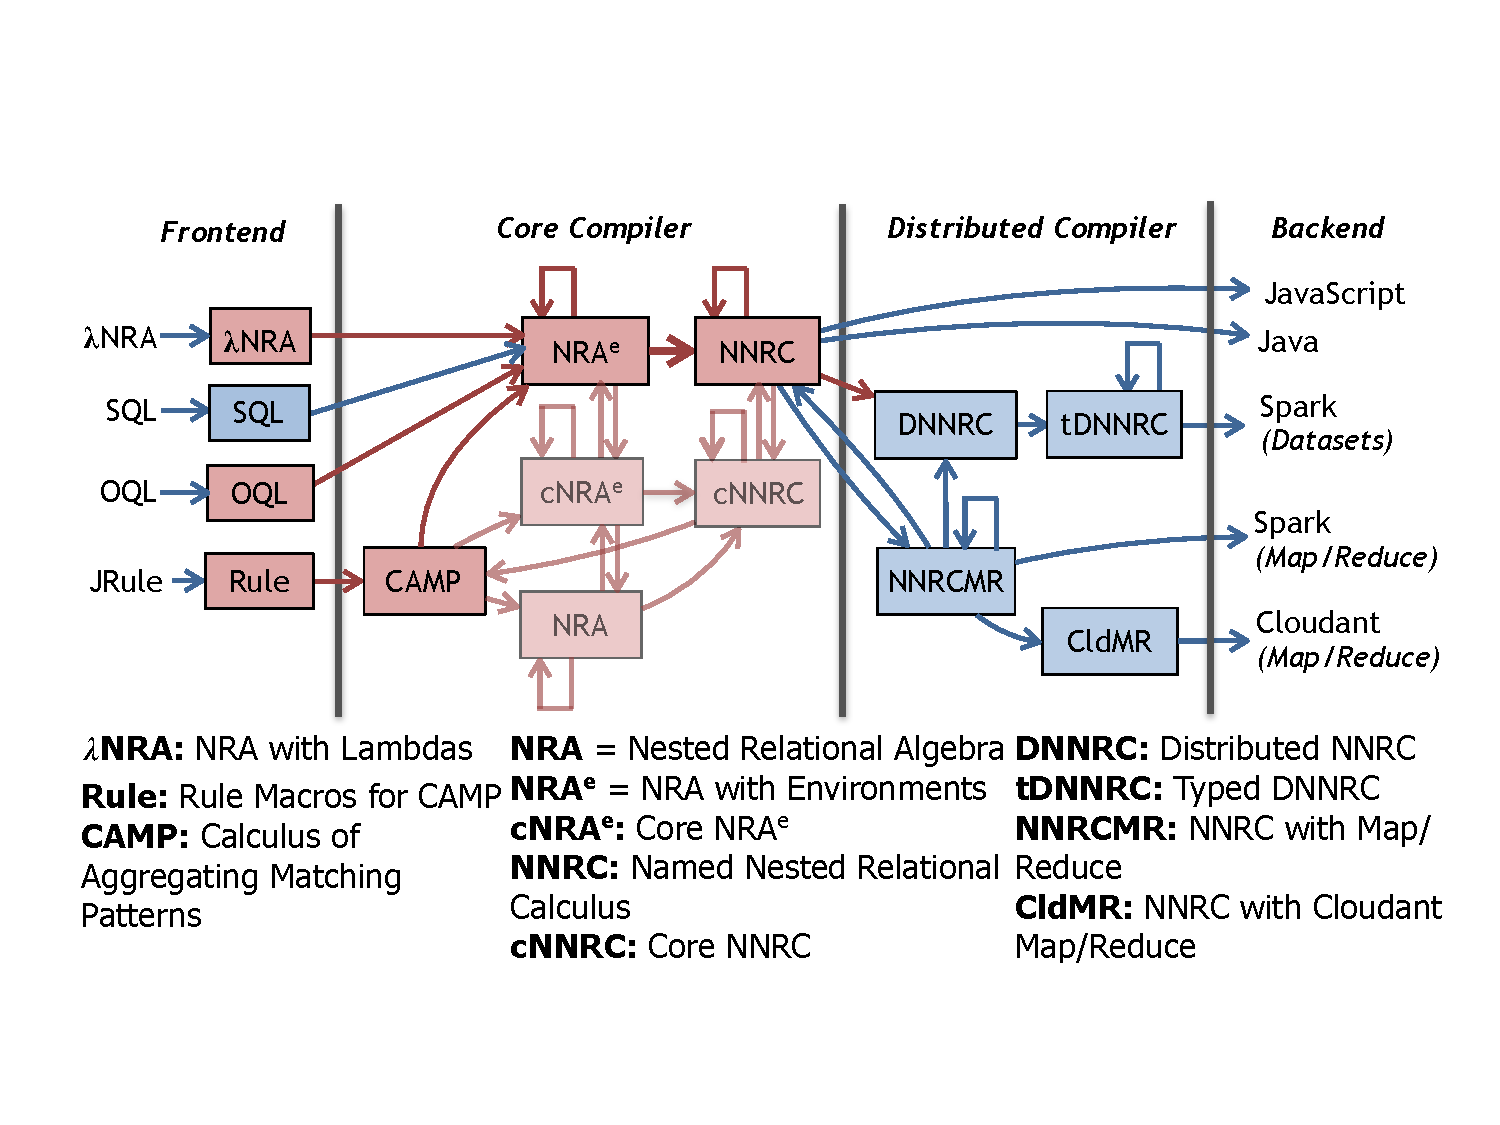
\includegraphics[width=0.48\textwidth]{qcert-pipeline.pdf}}
  \caption{\label{fig:architecture}Q*cert compiler architecture.}
\end{figure}

From a front-end perspective, the system includes a parser for OQL and
\NRALambda. JRules and SQL support rely on existing Java parsers for
those languages, which pass an AST to the compiler encoded as an
S-expression. The named nested relational calculus (NNRC) is the
gateway to the backend part of the compiler. It is directly used to
generate code for Java and JavaScript, while code generation for Spark
and Cloudant rely on additional intermediate representations (DNNRC
models distributed computation with Spark Datasets, NNRCMR models
map/reduce, and CldMR models Cloudant-specific map/reduce).

\paragraph*{Data model and type system}

In order to focus on the novel features of \NRAEnv, this paper uses a
simple data model of complex values with bags and records, and omits
the treatment of types. This is far from enough for practical
languages. For instance, OQL and JRules support class hierarchies, and all
our languages require support for null values, date comparisons, and
arithmetic. The implementation supports a rich data model that
includes a notion of objects as well as sum types in a way similar
to~\cite{GiorgidzeGUW12,WF2016}. The compiler specification and
correctness proofs are done over that richer data model and type
system. It is important to recall that type correctness is used
pervasively as a pre-condition for algebraic rewrites and rely on type
checking and type soundness proofs for the intermediate languages.

To handle additional data types (e.g., dates), and provide some
modularity, the mechanization is parameterized over a notion of
``foreign'' types and operators. From a Coq perspective, those are
\emph{axioms} that are assumed by the proof system. A set of axioms
for each foreign type typically includes semantics and typing
judgments, with correctness
properties\,\coqdef{Basic.ForeignRuntime}{}. When the compiler is
extracted, an \emph{implementation} of those axioms as regular code
must be provided. Note that this choice represents a trade-off, since
Coq cannot ensure the correctness of that part of the implementation.

\paragraph*{Optimizer}

Most of the formal treatment of the paper uses algebraic equivalences
to convey optimizations. As we mentioned in the introduction, those
are used as part of the proof of correctness for the optimizer
itself. These optimizations are written as individual pattern-match
based transformations (with side conditions as needed), each of which
is proven to preserve semantics (and typing as appropriate).

The optimization infrastructure is parameterized by a list of rewrites
and a cost function. All possible rewrites are applied through a
depth-first AST traversal and optimization proceeds as long as the
cost is decreasing.
%
Despite being simple by traditional databases standards, the optimizer
includes on the order of a hundred rewrites. The cost is currently
based on the size and depth of the query which means there is a lot of
room for improvements on that part of the implementation. Coq does not
introduce specific limitations as to the complexity of the optimizer,
which could use a search space and more complex cost model.

Finally, we have made some efforts to ensure that adding new
optimizations is relatively straightforward. As shown in the
introduction, each rewrite can be programmed and proved individually.
The infrastructure provides a tactic that helps with this, in order to
automatically reduce the full proof to a proof of the individual
type-directed rewrite.

\paragraph*{Support for other languages}

Our current compiler uses well-known database representations which
means it can easily be used to investigate or validate novel
optimizations for other use cases, as we have done for CAMP. The
amount of work required for adding a new language to the compiler
depends on the nature of the language. Q*cert makes a few important
assumptions: one is a data model based on nested relations, the other
is that type checking is assumed in most of the optimizer support. As
a result, the compiler should be a good match for Spark~(which we
partially support), Pig~Latin~\cite{OlstonRSKT08}, or JSON languages
such as Jaql~\cite{BeyerEGBEKOS11-full}. Additional work on typing for
semi-structured data would make languages such as
JSONiq~\cite{florescu2013jsoniq} or SQL++~\cite{OngPV14} interesting
next steps. Languages such as XQuery would require significant changes
to the compiler because of the complexity of the XML data model.

\paragraph*{Thoughts on Coq}

Coq is a functional programming language that fits well the task of
writing compilers. Proofs can be added gradually, extraction is
robust, and the code generated benefits from the good quality of the
OCaml compiler, both in terms of stability and performances. The
current performance bottlenecks in our implementation are in the
optimizers, which can lead to an exponential number of iterations over
the tree. However, it should be possible to use memoization techniques
to improve performances~\cite{braibant2014implementing}.

One of the pleasant surprises of our experience has been the
versatility of Coq, which we feel could be used to tackle a range of
database problems. For instance, similar techniques could be used for:
the specification of a query language after the fact or during
development (for documentation and prototyping), ensuring the
correctness of complex algorithms (e.g., view maintenance), or
building an end-to-end verified compiler. This last scenario
would certainly be a large undertaking and would require addressing
integration issues with a real database engine.

%%% Local Variables:
%%% TeX-master: "main"
%%% End:
